\documentclass[12pt,]{book}
\usepackage[]{tgpagella}
\usepackage{amssymb,amsmath}
\usepackage{ifxetex,ifluatex}
\usepackage{fixltx2e} % provides \textsubscript
\ifnum 0\ifxetex 1\fi\ifluatex 1\fi=0 % if pdftex
  \usepackage[T1]{fontenc}
  \usepackage[utf8]{inputenc}
\else % if luatex or xelatex
  \ifxetex
    \usepackage{mathspec}
  \else
    \usepackage{fontspec}
  \fi
  \defaultfontfeatures{Ligatures=TeX,Scale=MatchLowercase}
\fi
% use upquote if available, for straight quotes in verbatim environments
\IfFileExists{upquote.sty}{\usepackage{upquote}}{}
% use microtype if available
\IfFileExists{microtype.sty}{%
\usepackage{microtype}
\UseMicrotypeSet[protrusion]{basicmath} % disable protrusion for tt fonts
}{}
\usepackage[margin=1in]{geometry}
\usepackage{hyperref}
\hypersetup{unicode=true,
            pdftitle={Politics Among Rebels: The Causes of Division Among Dissidents},
            pdfauthor={David F. Bowden},
            pdfborder={0 0 0},
            breaklinks=true}
\urlstyle{same}  % don't use monospace font for urls
\usepackage{natbib}
\bibliographystyle{plainnat}
\usepackage{longtable,booktabs}
\usepackage{graphicx,grffile}
\makeatletter
\def\maxwidth{\ifdim\Gin@nat@width>\linewidth\linewidth\else\Gin@nat@width\fi}
\def\maxheight{\ifdim\Gin@nat@height>\textheight\textheight\else\Gin@nat@height\fi}
\makeatother
% Scale images if necessary, so that they will not overflow the page
% margins by default, and it is still possible to overwrite the defaults
% using explicit options in \includegraphics[width, height, ...]{}
\setkeys{Gin}{width=\maxwidth,height=\maxheight,keepaspectratio}
\IfFileExists{parskip.sty}{%
\usepackage{parskip}
}{% else
\setlength{\parindent}{0pt}
\setlength{\parskip}{6pt plus 2pt minus 1pt}
}
\setlength{\emergencystretch}{3em}  % prevent overfull lines
\providecommand{\tightlist}{%
  \setlength{\itemsep}{0pt}\setlength{\parskip}{0pt}}
\setcounter{secnumdepth}{5}
% Redefines (sub)paragraphs to behave more like sections
\ifx\paragraph\undefined\else
\let\oldparagraph\paragraph
\renewcommand{\paragraph}[1]{\oldparagraph{#1}\mbox{}}
\fi
\ifx\subparagraph\undefined\else
\let\oldsubparagraph\subparagraph
\renewcommand{\subparagraph}[1]{\oldsubparagraph{#1}\mbox{}}
\fi

%%% Use protect on footnotes to avoid problems with footnotes in titles
\let\rmarkdownfootnote\footnote%
\def\footnote{\protect\rmarkdownfootnote}

%%% Change title format to be more compact
\usepackage{titling}

% Create subtitle command for use in maketitle
\newcommand{\subtitle}[1]{
  \posttitle{
    \begin{center}\large#1\end{center}
    }
}

\setlength{\droptitle}{-2em}
  \title{Politics Among Rebels: The Causes of Division Among Dissidents}
  \pretitle{\vspace{\droptitle}\centering\huge}
  \posttitle{\par}
  \author{David F. Bowden}
  \preauthor{\centering\large\emph}
  \postauthor{\par}
  \predate{\centering\large\emph}
  \postdate{\par}
  \date{May 4, 2017}

\usepackage{setspace}


\usepackage{float}
\let\origtable\table
\let\endorigtable\endtable
\renewenvironment{table}[1][2] {
    \singlespacing
    \expandafter\origtable\expandafter[H]
} {
    \endorigtable
}

\begin{document}
\maketitle

{
\setcounter{tocdepth}{1}
\tableofcontents
}
\doublespacing

\chapter{Introduction}\label{introduction}

\section{Previous Work on the Structure of Rebel
Movements}\label{previous-work-on-the-structure-of-rebel-movements}

The existing literature and empirical record suggest that the number of
rebel groups active in a conflict is shaped by three broad processes.
The number of rebel groups can increase when existing groups splinter
into multiple factions. New groups can also emerge when previously
non-violent individuals mobilize and join the conflict. Finally, the
number of rebel groups can decrease when previously independent factions
form alliances. In the remainder of this chapter, I provide a definition
of each process, and review the existing explanations for each.

\subsection{Splintering}\label{splintering}

Existing rebel groups frequently splinter into multiple successor
organizations. In 1968, for example, a faction led by Ahmed Jibril broke
away from the Popular Front for the Liberation of Palestine (PFLP) to
form a new group, the Popular Front for the Liberation of
Palestine-General Command (PFLP-GC). While the two groups often
collaborated against Israel, they maintain distinct organizational
structures and membership bases, and operate in different areas. The
split was allegedly motivated by differing views of Marxist ideology and
military doctrine, with the PFLP pursuing a more extreme strategy of
attrition. Similar splits have occurred within dozens of rebel groups,
including the Communist Party of Burma, the Free Syrian Army and the
Sudan Liberation Army. In many cases the result is more than a nominal
separation. In Sri Lanka, for example, the Tamil Peoples Liberation
Tigers not only split from the Liberation Tigers of Tamil Eelam, but
also defected to the government side in the conflict
\citep{Staniland2012d}.

A growing body of literature identifies several key determinants of
rebel group splintering. One subset of this research focuses on the role
of external actors, and particularly the government. For instance,
\citet{McLauchlin2012} find that government repression provides occasion
for groups to evaluate their current leadership structure. Pre-existing
divisions within groups are likely to be exacerbated, leading the group
to move toward more factionalized leadership structures. When group
members are satisfied, however, conflict tends to lead to even greater
unity and centralization of authority. Whereas the preceding studies
essentially treat government repression as exogenous to the internal
politics of dissident groups, \citet{Bhavnani2011} present evidence that
governments deliberately stoke tensions among their opponents, as they
find that the Israeli government increased conflict between Fatah and
Hamas by undermining Hamas' control of the Gaza and by tolerating
Fatah's relationship with the Jordanian military.

Another group of scholars emphasizes concerns about post-conflict
bargaining as the key determinant of dissident group cohesion.
\citet{Christia2012} assumes that the winning coalition in a civil war
receives private benefits, which might include any rents available to
the state, and having some portion of its interests represented in the
new government. Thus, rebels have an incentive to form minimum winning
coalitions, so as to limit the number of coalition partners with whom
they must share benefits. \citet{Wolford} develop a similar logic,
theorizing that political factions have an interest in joining conflicts
so as to maximize the likelihood of their preferences being represented
in the post-war government, but the value of fighting decreases as the
number of parties with whom they expect to share power increases. Yet,
\citet{Christia2012} suggests that this incentive to minimize coalition
size is moderated by the risk of being outside the winning coalition, as
there is a strong possibility of new waves of violence between
victorious rebels and rival rebel factions. She thus expects coalitions
to change frequently in response to battlefield events, with factions
bandwagoning with battle winners and shifting away from losing
coalitions. \citet{Findley2012} similarly find fragmentation to be most
common among groups that have recently lost battles. This implies that
fragmentation is essentially a process of weak actors becoming weaker.

A final category of explanations places the source of rebel group
cohesion in underlying social structure. \citet{Staniland2014} argues
that insurgent organizations will be most stable when their central
leadership is able to exercise both vertical control over its
rank-and-file members, and horizontal control over its constituent
groups. This is most likely to occur when insurgencies draw from
existing organizations with extant social ties of this sort, which might
include former anti-colonial movements or ethnic political parties.
Organizations are likely to fragment when constituent groups have a high
degree of autonomy or control over individual members is limited
\citep[Ch. 2-3]{Staniland2014}. \citet{Asal2012} emphasize similar
factors, arguing that organizations with factionalized leadership
structures are at risk of fragmentation, while groups with more
consolidated power structures will tend to remain cohesive. Finally,
\citet{Warren2015} suggest that group size plays an important role, as
small groups are able to police themselves and resolve conflicts,
whereas larger groups are more likely to experience infighting.

Each of these studies makes an important contribution to our
understanding of conflict complexity, and sheds light on the broader
interests and organizational challenges present in rebel movements. Yet,
while the fragmentation of existing groups accounts for a substantial
portion of multi-rebel conflicts, other processes are at work in the
majority of cases. Indeed, only 26.6\%\footnote{These figures are
  calculated using data on conflict participation from
  \citet{Pettersson2015a} and actor attributes from \citep{ucdpactor}. I
  code a conflict episode as a separate war if it occurs following at
  least two calendar years of inactivity. Secessionist movements are
  treated as separate conflicts from bids to overthrow the central
  government, and separate from each other if they concern different
  territories.} of the rebel groups that join ongoing civil wars
splintered from an existing group, and only 9.7\% are agglomerations of
existing groups. Thus, nearly two-thirds of the groups that join
conflicts\footnote{The pattern is even more stark if one looks at
  conflict-years, as over 95\% of conflict years with multiple
  government-rebel dyads include at least one rebel group that is
  neither a splinter organization nor the source of one.} (only 20\% of
multi-dyadic conflicts have multiple rebel groups from the outset) do
not appear to be the product of existing combatants reconfiguring, but
rather are the result of an entirely new group of combatants entering
the fray. I propose an integrated approach that accounts for both the
fragmentation of existing groups, and the entry of new groups to the
conflict.

\subsection{Alliance Formation}\label{alliance-formation}

Several studies consider alliance formation among terrorist
organizations.

\subsection{Mobilization}\label{mobilization}

Few, if any, studies directly consider the phenomenon of new rebel
groups joining ongoing conflicts. The literature on contagion is perhaps
most relevant. \citet{Gleditsch2007} finds that transnational ethnic
groups and political and economic linkages between states can provide
channels for civil war to spread across international boundaries. Other
scholars find that secessionist \citep{Ayres2000} and ethnic
\citep{Lane2016} conflict often spread through processes of contagion,
with the rebellion of one group seemingly inspiring those in neighboring
areas to take up arms themselves. Such transnational processes might
shape opportunities for multiple rebellions to emerge by increasing the
availability of weapons, spreading tactical knowledge, or diverting
government attention to foreign conflicts. Similarly, transnational
motives for conflict may come in the form of grievances becoming clearer
and more salient in light of events in neighboring countries, as
happened during the Arab Spring, or the expected probability of a
successful rebellion shifting upward in response to nearby events. Yet,
rebel groups that are themselves transnational, operating in multiple
countries {[}see{]} \citet{salehyan07}{]} account for only 10.8\% of
conflict joiners.

\chapter{The Entry of New Groups}\label{the-entry-of-new-groups}

\section{Introduction}\label{introduction-1}

Why do some civil wars have multiple rebel groups, while others have
only one? Theories of civil war tend to focus on individual- or
group-level motives \citep[e.g.][]{gurr70, Collier2004} or opportunities
\citep[e.g.][]{fearonlaitin03} for rebellion, while giving little
attention to the organization of dissent into rebel groups and
coalitions. Even those studies which do explicitly consider rebel group
formation tend to focus on group attributes such as treatment of
civilians \citep[e.g.][]{Weinstein2007}, and do not consider the
possibility that rebels do not always form a single group. Yet, at least
two rebel groups are active at some point in 44\% of civil
conflicts.\footnote{Source: \citet{Pettersson2015a}.} Over the course of
the Chadian Civil War, for instance, 25 distinct rebel groups fought
against the government at various times. Conflicts in Afghanistan in the
1980's, Somalia in the 1990's, Sudan in the 2000's have been similarly
complex. The ongoing civil war in Syria is contested by at least two
dozen armed groups. Even ethnically-homogeneous,
geographically-concentrated populations with common goals, such as the
Karen secessionist movement in Myanmar, often fragment into multiple
rebel groups. Furthermore, the number of groups operating in these
conflicts often varies greatly over time. The existing literature offers
many useful insights to the conditions under which civil war will
emerge, but it has relatively few explanations for the structure of
rebel movements. The studies that do address some aspect of the
phenomenon focus overwhelmingly on the fragmentation of existing groups
\citep[e.g.][]{McLauchlin2011, Christia2012, Staniland2014}, and do not
consider the mobilization of entirely new groups. I thus address the
question: why do rebel groups join ongoing civil conflicts?

While little attention has been given to the sources of rebel movement
structure, several studies suggest that fragmented rebel movements are
associated with particularly concerning conflict attributes. Conflicts
with multiple rebel groups last longer than dyadic competitions
\citep{Cunningham2006, Cunningham2009, Akcinaroglu2012a}. Furthermore,
\citet{Cunningham2009} find that the presence of multiple
government-rebel dyads decreases the likelihood of peace agreements and
increases the likelihood of rebel victories, though \citet{Findley2012},
find that fragmented rebel movements are often associated with an
\emph{increased} likelihood of negotiated settlement. Relatedly,
\citet{Atlas1999} and \citet{Zeigler2016} find that episodes of conflict
renewal often occur between formerly allied rebel factions. Finally,
conflicts with multiple dyads feature more fatalities than dyadic
ones.\footnote{Source: my own analysis using data from
  \citet{Sundberg2008a}.} Clearly, conflicts with multiple rebel groups
comprise one of the most severe subsets of civil wars. Thus,
understanding the causes of multi-dyadic conflict is of great normative
and policy importance.

This work contributes to the existing literature by advancing our
understanding of the complexity of civil conflict in terms of the number
of warring parties. In doing so it builds on the growing literature on a
related facet of complexity --- the fragmentation of existing groups
\citep[see][]{Cunningham2009, Pearlman2011a, Staniland2014}.
Furthermore, examining the relationships between rebel groups sheds new
light on debates about the motives behind rebellion
\citep[e.g.][]{Collier2004}. For instance, if rebellion is fundamentally
about ethnic or religious grievances as recent works have asserted
\citep{Cederman2010}, we might expect to see such concerns influence the
structure of rebel coalitions as well. If, by contrast, rebels are
motivated by the desire for profits from natural resources or illicit
activities, the propensity for new groups to enter conflicts would
likely be related to the availability of such resources, and not to
political context. Finally, as my theory emphasizes the role of
repression in incentivizing new actors to join the conflict, it builds
on existing work on wartime civilian targeting
\citep[e.g.][]{Kalyvas2006} to show that repression can shape not only
whether individuals elect to join conflicts, but also how they organize
themselves when choosing to do so.

I proceed by elaborating a theoretical framework for studying the
processes that might lead new rebel groups to join an ongoing civil
conflict. Next, I argue that targeted repression is an especially
influential force in producing new rebel groups, as it both reduces the
relative cost of fighting, and induces individuals to identify more
strongly with sub-national groups. After outlining a research design, I
use fixed-effects poisson regressions to model the number of rebel
groups competing in civil wars worldwide between 1946 and 2015, finding
support for my hypotheses. Finally, I summarize the implications of the
findings and identify several opportunities for further research.

\section{Theoretical Framework}\label{theoretical-framework}

Broadly, a conflict can come to have multiple rebel groups through two
processes - the splintering of existing groups into multiple successor
organizations, and the formation of an entirely new organization by
previously non-violent individuals. At a minimum, then, the creation of
new rebel groups requires division among the dissidents who comprise the
pool of current and potential rebels. Splinter factions must have a
reason for leaving their parent organization, and newly mobilizing
individuals must have a reason for forming a new group rather than
joining an existing one. At their most benign, these divisions might
simply reflect the difficulty of coordinating actions across physical
distance or linguistic barriers. In such cases the formation of multiple
rebel groups might be a matter of convenience rather than an indicator
of animosity or divergent objectives. In other cases, however, divisions
may be deeper and more difficult to reconcile. For instance, if some
rebels make improving the status of their ethnic group a primary
concern, it is unlikely that members of other ethnic groups will join
their organization, and any existing members with differing ethnic
identities will be likely to leave.

\begin{longtable}[]{@{}ll@{}}
\caption{Necessary Conditions for the Formation of New
Groups}\tabularnewline
\toprule
Splinter Group & Entirely New Group\tabularnewline
\midrule
\endfirsthead
\toprule
Splinter Group & Entirely New Group\tabularnewline
\midrule
\endhead
Division among dissidents & Division among dissidents\tabularnewline
& Change in relative value of fighting\tabularnewline
\bottomrule
\end{longtable}

In addition to divisions with existing groups, the formation of new
groups requires that previously non-violent individuals change their
mobilizational calculus. This entails either participation in violence
becoming more attractive, or remaining non-violent becoming less
attractive. The former might occur in situations where an individual
found the grievances that led to the initial violence insufficiently
persuasive to justify fighting, but new, more persuasive grievances
emerge. For example, violence against civilians might lead new
dissidents to mobilize in response. Alternatively, the initial fighting
might reveal the government to be weaker than perviously thought,
leading some to reconsider their decision to abstain from fighting.
Non-violence can become less attractive if, for example, the conflict
disrupts economic activity, decreasing the opportunity cost of fighting
\citep[see][]{Collier1998}. Indiscriminate violence against civilians
can have similar effects by reducing the the risk of participation in
violence relative to that of non-violence \citep{Kalyvas2007}. If the
physical risk of remaining peaceful is not dramatically lower than that
of fighting, the cost of participating in rebellion is relatively low.
In the following sections, I argue that government repression,
particularly when targeted at specific ethnic groups, can satisfy both
requirements for the formation of new rebel groups --- repression
reduces the relative cost of fighting, and targeted repression
activiates social identities that can sow division among dissidents.

\subsection{The Perils of Ethnic
Politics}\label{the-perils-of-ethnic-politics}

Rebellions are organized around a variety of identities, ideologies, and
goals. The Communist Party of India advocates a Marxist-Leninist
ideology, Darul Islam sought to establish an Islamic state in Indonesia,
the National Forces of Liberation challenged the ruling Tutsi minority
in Burundi on behalf of ethnic Hutus, and the Kurdistan Democratic Party
backs an irredentist goal of creating an independent Kurdish state in
parts of Iraq, Syria, and Turkey. Many scholars have argued that ethnic
identities are a particularly useful basis for mobilization. Ethnic
groups tend to be among the most salient identities in society, and thus
serve as a focal point for mobilization \citep{Hardin1995, Hechter2001}.
Furthermore, coethnics often have overlapping social networks, meaning
that their interactions occur under the shadow of the future, mitigating
many barriers to cooperation \citep{Habyarimana2012}. Indeed, several
empirical studies find that ethnically-homogeneous groups are better
able to cooperate than more diverse ones
\citep{Alesina1999, Miguel2005, Habyarimana2012}. Yet while activating
ethnic identities may be advantageous for the initial organization of
rebellion, I argue that in diverse societies such identities can have
deleterious effects on the cohesion of rebel movement.

Intra-ethnic politics often follows a dynamic known as ``outbidding,''
in which leaders make progressively more extreme proposals in hopes of
winning the support of the group \citep{Rabushka1972, horowitz85}. Key
to these models are the assumptions that individuals identify with a
single ethnic group, that they care only about ethnic issues, and that
ethnic politics is a zero-sum game. This produces a completely polarized
bargaining space in which individuals hold positions on ethnic issues in
which their group's interests are represented fully (e.g.~a preference
for a legislature in which group members hold a majority). In a spatial
model of voting with such parameters, the optimal strategy for
politicians is to adopt the most extreme position possible
\citep{Rabushka1972}. Even if a multi-ethnic coalition forms initially
by creating uncertainty as to which group will be advantaged, it will
eventually be undercut by challengers making more extreme appeals to one
ethnic group. Other bases of mobilization, by contrast, tend to produce
more heterogenous preferences - some members will actually prefer
moderate positions - and thus greater potential for compromise. While
the original formulation of the outbidding model assumes competition in
an electoral context, it has also been shown to more violent forms of
competition such as terrorism
\citetext{\citealp{Kydd2006}; \citealp{Chenoweth2010}; \citealp[but
see][]{Findley2012a}}.

Adding to the zero-sum character of competition between ethnic groups is
the fact that ethnic rebellions are far more likely than others to claim
specific pieces of territory. Ethnic rebellions often make secessionist
or irredentist claims against the government, while such demands are
relatively rare among multi-ethnic rebellions in the post-colonial era.
Territorial division is a zero-sum game - any territory gained by the
secessionist movement comes at the expense of the state, and vice-versa.
Furthermore, while in theory territory can be divided, resulting in
compromise solutions, in fact it often takes on symbolic importance that
renders it indivisible \citep{Toft2003}. In addition to creating the
zero-sum dynamic between an ethnic group and the state common to many
ethnic issues, territorial claims can generate competition between
different ethnic groups. Many territories are claimed by multiple ethnic
groups \citep{Toft2003}, placing secessionist claims into competition.
Even in the absence of symbolic value, the territories that form
secessionist claims are often remote, making them attractive bases for
all rebel groups \citep{Fjelde2012}. The activation of ethnic identities
should thus create difficult-to-resolve competitions between dissidents
of differing ethnicities, ultimately leading to an increase in the
number of factions competing in a civil war.

\subsection{Repression and the Dynamics of
Identity}\label{repression-and-the-dynamics-of-identity}

Some theoretical perspectives view ethnic and other social identities as
largely immutable, deriving from ancient histories \citep{horowitz85}.
Increasingly, however, scholars view identity as a product of individual
or collective choice. \citet{Posner2005} argues that individuals choose
to prioritize one of several identities such as ethnicity, language,
religion, or class, selecting that which is likely to bring them the
greatest benefit. Focusing on the realm of electoral politics, he finds
that this choice is shaped by an interaction between group size and
electoral institutions. In subsequent work \citet{Eifert2010} find that
individuals are more likely to identify with their ethnic group when
interviewed near a competitive election. \citet{Penn2008} models a
similar calculation in which individuals choose to orient themselves
toward a national or ethnic identity. She finds that ethnic identities
become more prevalent as ethnic groups become homogenous, and as
economic inequality between ethnic groups increases.
\citet{Christia2012} extends the argument to civil wars, arguing that
ethnic identities are deployed instrumentally, with rebel elites
emphasizing particular identities to justify alignments that are in fact
driven by power politics. A key consequence of this malleability of
identity is that ethnic outbidding is not inevitable - if political
actors can appeal to multiple, overlapping identities, competition is no
longer zero-sum \citep{Chandra2005}. The opposite is also true, however
- previously cooperative relationships can be undermined by enhancing
the salience of ethnic identities.

I argue that selective repression - repression which is targeted at
certain individuals or groups while sparing others - should tend to
increase the number of rebel groups in a conflict both by decreasing the
relative cost of violent mobilization and by increasing the salience of
particular identities. Indiscriminate repression, by contrast, should
not systematically decrease the cohesiveness of dissident movements.
First, repression should have a general effect of increasing the number
of individuals participating in a conflict. Some individuals will
participate in violence even when doing so comes at high cost. Many,
however, will only participate when the cost of doing so is low relative
to the cost of remaining non-violent. As one of the primary costs of
participation in rebellion is the risk of physical harm, repression
should tend to reduce the relative cost of rebellion by bringing the
risk of physical harm to non-violent activities. Any form of repression
should thus increase the number of individuals in a country willing to
participate in violence.

\emph{Hypothesis 1: The number of rebel groups in a country should
increase with the level of repression}

The effect of repression on the structure of rebel movements, however,
should depend on its form. While indiscriminate repression that targets
many individuals within society should expand the pool of individuals
willing to participate in rebellion, it should not systematically affect
their desire to form new groups rather than joining existing ones. Some
individuals may turn to an ethnic or religious group for protection, but
in other cases widespread repression may unify citizens in opposition to
their government. For example, the citizens of many former colonies
banded together to pursue independence, before subsequently fragmenting
along ethnic lines. Thus while indiscriminate repression should in some
cases lead to an increased number of rebel groups, the aggregate effect
should be of moderate strength.

In comparison, indiscriminate repression should be far more likely to
increase the number of rebel groups in a conflict, as it induces
individuals to identify with particular subnational groups. While
targeted repression can be done on the basis of support for existing
rebels \citep{Kalyvas2006}, often it is done on the basis of ethnicity
or religion. For example, the Myanmarese government has frequently
repressed the Rohingya ethno-religious minority, while being
considerably more repsectful of the rights of the Burman majority. I
focus on this sort of targeted repression. When individuals are targeted
on the basis of group membership, these groups are likely to increase in
salience relative to other social cleavages. Furthermore, individuals
are highly likely to develop a sense of linked fate with fellow group
members. In other words, they are likely to adopt the belief that their
prosperity and perhaps even survival depends on their ability to band
together and defend themselves. Thus, targeted repression should lead
individuals to mobilize on the basis of the targeted group. Unless an
existing rebel group was already mobilized on such a basis, this should
result previously non-violent individuals forming new groups, and in
members of existing groups forming splinter organizations that emphasize
their identity.

\emph{Hypothesis 2: The number of rebel groups in a country should
increase with the extent to which repression is discriminatory}

In statistical terms, I expect that the relationship between repression
and discrimination to be interactive, rather than additive. That is, I
expect the effect of increasing the severity repression on the number of
rebel groups to be very strong when it is targeted (discriminatory), and
more modest when it is deployed indiscriminately. I expect the reverse
to hold as well --- the effect of discrimination should be greater when
as severity of repression increases. While targeted, but weak repression
might enhance ethnic identities, I do not expect that it will
dramatically alter the relative cost of fighting. In short, I expect to
find a statistically significant, positive interaction term.

\emph{Hypothesis 3: There is a positive interactive effect between the
level repression and the extent to which repression is discriminatory}

\section{Research Design}\label{research-design}

To test the preceding hypotheses I use a dataset of country war-years
derived from the Uppsala Conflict Data Program and Peace Research
Institute Oslo's Dyadic Dataset, version 4-2016
\citep{Harbom2008, Melander2016}. This dataset includes one observation
for every government-rebel group dyad for each year in which it produced
at least 25 fatalities. I excluded all interstate conflicts from the
data, and include all civil wars, anti-colonial wars, and
internationalized civil wars. I then aggregate this data to the
country-year, producing a count of the number of rebel groups active in
each country experiencing a civil war each year. This results in a
dataset of 1,501 observations, covering the period 1946--2015. Note that
the UCDP data typically allows for the presence of multiple conflicts
within the same country-year --- rebel groups pursuing secession are
considered part of a separate conflict from rebels challenging the
central government, and rebels pursuing secession for different
territories are considered separate from one another. I ignore these
distinctions and aggregate to the country-year for two reasons. First,
my theory focuses largely on the role of government behavior in shaping
rebel structure, and thus it makes sense to group all rebels facing the
same government together. From the government's standpoint, beyond a
tactical level it may make little difference whether a new rebel group
is challenging the central government or pursuing secession --- both
outcomes are undesirable. Second, most of my independent variables are
measured at the country level, and in many cases it would be difficult
to record subnational variation, particularly in a dynamic fashion.

\subsection{Dependent Variables}\label{dependent-variables}

\begin{itemize}
\tightlist
\item
  \textbf{Number of Rebel Groups} My primary dependent variable is the
  number of rebel groups active in a country-conflict-year. The data
  comes from the UCDP Dyadic data \citep{Harbom2008, Melander2016},
  which considers rebel factions to be separate groups if they have a
  discernible name. In other words, a faction connected to a larger
  group would be considered an independent organization and count toward
  this measure if it had its own name; otherwise, it would be considered
  part of the larger organization. Name \emph{changes}, however, only
  result in the entry of a new group to the data if they are accompanied
  by a substantial change to the organization's composition such as a
  merger with another group. Note that given the difficulties of
  determining precisely when many rebel groups ceased operations, this
  measure includes all groups that appear at any point during the
  calendar year; it is therefore possible that this measure overstates
  the number of groups that were active simultaenously in some cases.
\item
  \textbf{Number of Non-Splinter Rebel Groups} As the process by which
  entirely new rebel groups emerge is likely to be somewhat different
  than the process by which existing rebel groups splinter, I employ an
  alternate DV that excludes splinter organizations from the count of
  active rebel groups. The measure is based on my own data collection on
  rebel origins, with groups being coded as splinter organizations if
  their leader and majority of members were previously part of a
  different rebel group, and transitioned directly to operating as an
  independent group (i.e.~there was no period of peace between
  membership in the previous and new organizations).
\end{itemize}

\subsection{Independent Variables}\label{independent-variables}

\begin{itemize}
\tightlist
\item
  \textbf{Human Rights} To measure repression I use the Latent Human
  Protection Scores, version 2 \citep{Fariss2014, Schnakenberg2014}.
  This data uses a Bayesian measurement model to estimate latent human
  rights scores using several data sources including US State Department
  and Amnesty International country reports, and several scholarly
  datasets on repression and mass killing. This data improves on
  previous approaches to measuring human rights by accounting for the
  fact that the standards by government and NGO reports have judged
  countries have generally improved over time. The result is an
  aggregate measure that ranges from roughly -3 (most repressive) to 3
  (most respectful of human rights). Within my data the mean score is
  -1.19, and no country year has a score higher than 1.51. This measure
  is lagged by one year.
\item
  \textbf{Discrimination} Currently, all major human rights data is
  measured at the country level. A direct measure of the extent to which
  repression is targeted at specific ethnic groups, geographic locales,
  etc. is thus unavailable. I use a measure constructed from the Ethnic
  Power Relations Core dataset, 2014 version \citep{Vogt2015}. EPR codes
  the political status of each politically-relevant ethnic group in the
  world, as well as several group attributes including their size as a
  percentage of the population. I consider groups coded as
  ``Discriminated'' or ``Powerless'' to be the victims of
  discrimination, and use the group size measure to calculate the
  percentage of the total country population that is subjected to
  discrimination. To aid in interpretation, I use the percentage of the
  country that is \emph{not} subjected to discrimination in the models.
  Thus, as the measure increases, the extent to which repression is
  targeted at a small minority increases. The rare cases where no
  members of society experience discrimination are recoded to 0, as this
  indicates a non-discriminatory regime. This measure is lagged by one
  year.
\end{itemize}

\subsection{Control Variables}\label{control-variables}

\begin{itemize}
\tightlist
\item
  \textbf{Conflict Intensity} To account for the possibility that human
  rights scores are simply a function of conflict intensity, rather than
  discriminatory intent, I include the maximum Conflict Intensity value
  from the UCDP Dyadic data. The measure is binary, with a value of 1
  indicating that the dyad produced between 25 and 999 fatalities in a
  given year, and a value of 2 indicating that the dyad produced 1,000
  or more fatalities. This measure is moderately correlated with the
  human rights score (Pearson's r = -0.30).
\item
  \textbf{Number of UCDP Conflicts} I include the number of distinct
  UCDP conflicts in a country-year as a control. Recall that all rebels
  challenging the central government are coded as being part of the same
  conflict, but each territory that is subject to a secessionist
  movement is considered distinct.
\item
  \textbf{Percentage Territorial Conflicts} To control for the
  possibility that secessionist conflicts produce different rebel
  structures, I include percentage of UCDP conflicts in a country-year
  that are fought over territory rather the central government.
\item
  \textbf{Neighboring Civil War} One potential mechanism that might
  produce increased numbers of rebel groups in a conflict is the
  movement of groups from neighboring countries into new conflicts. To
  control for this possibility I construct an indicator for the presence
  of a civil war in a neighboring state using the UCDP Dyadic data and
  the Correlates of War Direct Contiguity data, version 3.2
  \citep{Stinnett2002a}.
\item
  \textbf{Ethnolinguistic Fractionalization} To control for the
  possibility that simple ethnic diversity, rather than the repression
  of particular ethnic groups, accounts for the number of rebel groups
  in a country, I include a measure of ethnolinguistic fractionalization
  from \citet{fearonlaitin03}. The measure represents the probability
  that two randomly selected individuals from a country will speak
  different languages.
\item
  \textbf{Logged Population} Conceivably, the number of rebel groups in
  a country might simply be a function of the country's size. I thus
  control for the logged population of the country using data from
  \citet{Gleditsch2002b}.
\item
  \textbf{Logged GDP per capita} Economic development correlates with a
  variety of important political outcomes, including the onset of civil
  war. I include the logged per capita GDP of each country, with data
  again from \citet{Gleditsch2002b}.
\end{itemize}

Additionally, I have examined the effect of several other control
variables. None were statistically significant, nor did they
substantially alter the performance of my variables of interest. Thus, I
excluded them from the models reported below. This included several
country-level variables, as well as several attributes of the largest
rebel group active in a country-year.

\begin{itemize}
\tightlist
\item
  \textbf{Democracy} A binary indicator for countries with a Polity IV
  score greater than 5 \citep{Marshall2012}.
\item
  \textbf{Mountainous Terrain} A measure of the percentage of land in a
  country that is mountainous \citep{fearonlaitin03}.
\item
  \textbf{Oil Revenue} A binary indicator of whether one-third or more
  of a country's exports come from fossil fuels \citep{fearonlaitin03}.
\item
  \textbf{Previous Conflict} A binary indicator of whether the country
  had experienced a previous episode of conflict separated by at least
  three calendar years with no fighting reaching the 25 fatality
  threshold.
\item
  \textbf{Rebel Group Central Control} A binary indicator of whether the
  largest rebel group active during a conflict year had a centralized
  control structure \citep{Cunningham2013}.
\item
  \textbf{Rebel Group Political Wing} A binary indicator of whether the
  largest rebel group active during a conflict year had a political wing
  \citep{Cunningham2013}.
\item
  \textbf{Rebel Group Stronger} A binary indicator of whether the
  largest rebel group active during a conflict year was stronger than
  the government \citep{Cunningham2013}.
\item
  \textbf{Rebel Presence in Other States} A binary indicator of whether
  the largest rebel group active during a conflict year had a presence
  in other states \citep{Cunningham2013}.
\item
  \textbf{Rebel External Support} A binary indicator of whether the
  largest rebel group active during a conflict year was received any
  form of support from an outside government \citep{Cunningham2013}.
\item
  \textbf{Multi-Ethnic Rebel Group} An indicator of whether a rebel
  group draws support from more than one ethnic group, constructed from
  the ACD2EPR version 4-2014 dataset \citep{Vogt2015}.
\end{itemize}

\subsection{Statistical Model}\label{statistical-model}

As the dependent variable in this study is a count of rebel groups,
Ordinary Least Squares regression would be inappropriate. A Cameron and
Travedi test shows no evidence of overdispersion in any model
specification, meaning that Poisson regression is an appropriate model,
rather than negative binomial. I include fixed effects for both country
and year. However, the time fixed effects do not substantially alter the
results, and I exclude them frmo the models presented here.
Additionally, I cluster the standard errors by country.

\section{Results}\label{results}

The poisson regression results are reported in Table 2. Models 1 and 2
use a dependent variable that includes all rebel groups active in a
given year. Models 3 and 4 exclude splinter organizations. The ``Human
Rights'' coefficient in Model 1 provides a test of \emph{H1} which
predicted that the number of rebel groups should increase with the level
of repression. I am able to reject the null hypothesis of no
relationship between repression and the number of rebel groups, as the
latent respect for human rights measure has a negative relationship that
is statiscally signficant at the 99.9\% level. As respect for human
rights improves, the expected number of rebel groups declines. As a
country becomes more repressive, by contrast, the expected number of
rebel groups increases. Model 3 shows similar results (though only at a
95\% significance level), suggesting that the relationship is not driven
by the fragmentation of existing groups, but rather includes the
mobilization of many new groups. Substantively, the effect of repression
is large. As Figure 1 shows, the predicted number of rebel groups at the
most repressive end of the spectrum is roughly 3. In the country-years
where respect for human rights is highest (moderately high, in absolute
terms), the expected number of groups is around 1.

\begin{table}
\begin{center}
\begin{tabular}{l c c c c }
\hline
 & Model 1 & Model 2 & Model 3 & Model 4 \\
\hline
Intercept                         & $-2.17^{***}$ & $-2.03^{***}$ & $-15.19^{***}$ & $-15.09^{***}$ \\
                                  & $(0.59)$      & $(0.60)$      & $(0.71)$       & $(0.85)$       \\
Human Rights                      & $-0.26^{***}$ & $-0.08$       & $-0.27^{***}$  & $-0.15^{*}$    \\
                                  & $(0.03)$      & $(0.05)$      & $(0.04)$       & $(0.07)$       \\
Discrimination                    & $0.40^{***}$  & $-0.00$       & $0.43^{**}$    & $0.15$         \\
                                  & $(0.11)$      & $(0.11)$      & $(0.14)$       & $(0.20)$       \\
Human Rights X Discrimination     &               & $-0.31^{***}$ &                & $-0.19$        \\
                                  &               & $(0.08)$      &                & $(0.10)$       \\
Intensity Level                   & $0.01$        & $0.02$        & $0.17^{***}$   & $0.17^{***}$   \\
                                  & $(0.03)$      & $(0.03)$      & $(0.04)$       & $(0.04)$       \\
Number of Conflicts               & $0.38^{***}$  & $0.38^{***}$  & $0.33^{***}$   & $0.33^{***}$   \\
                                  & $(0.02)$      & $(0.02)$      & $(0.02)$       & $(0.02)$       \\
\% Conflicts Over Territory       & $-0.22^{***}$ & $-0.21^{***}$ & $-0.26^{***}$  & $-0.25^{***}$  \\
                                  & $(0.05)$      & $(0.05)$      & $(0.07)$       & $(0.07)$       \\
Logged GDP per capita             & $0.10^{**}$   & $0.10^{**}$   & $-0.10^{*}$    & $-0.10^{*}$    \\
                                  & $(0.03)$      & $(0.03)$      & $(0.05)$       & $(0.05)$       \\
Ethnolinguistic Fractionalization & $-1.21^{***}$ & $-1.42^{***}$ & $-0.21$        & $-0.33$        \\
                                  & $(0.28)$      & $(0.29)$      & $(0.42)$       & $(0.42)$       \\
Contiguous Civil War              & $0.02$        & $0.01$        & $-0.01$        & $-0.01$        \\
                                  & $(0.04)$      & $(0.04)$      & $(0.05)$       & $(0.05)$       \\
Logged Population                 & $0.07$        & $0.09$        & $-0.14^{*}$    & $-0.13$        \\
                                  & $(0.05)$      & $(0.05)$      & $(0.07)$       & $(0.07)$       \\
\hline
AIC                               & 3084.14       & 3082.34       & 2828.59        & 2829.58        \\
BIC                               & 3503.30       & 3506.55       & 3247.75        & 3253.79        \\
Log Likelihood                    & -1459.07      & -1457.17      & -1331.30       & -1330.79       \\
Deviance                          & 210.38        & 206.59        & 406.70         & 405.69         \\
Num. obs.                         & 1153          & 1153          & 1153           & 1153           \\
\hline
\multicolumn{5}{l}{\scriptsize{$^{***}p<0.001$, $^{**}p<0.01$, $^*p<0.05$}}
\end{tabular}
\caption{Poisson Regression Models of Rebel Group Count}
\label{table:coefficients}
\end{center}
\end{table}

Models 1 and 3 also provide tests of \emph{H2}, which expects that the
number of rebel groups should increase with the extent to which
repression is targeted in a discriminatory fashion. Again I am able to
reject the null hypothesis, as the effect of discrimination is positive
and statistically significant at the 99.9\% level in Model 1, and at the
99\% level in Model 3. As the percentage of a country's population that
is \emph{not} subjected to discrimination (i.e.~discrimination becomes
more targeted), the expected number of rebel groups increases. The
substantive effect is smaller than that for Human Rights, however (see
Figure 1). Moving from perfectly indiscriminate policies to the most
finely targeted increases the expected number of rebel groups from
roughly 1.4 to slightly over 2.

\begin{figure}
\centering
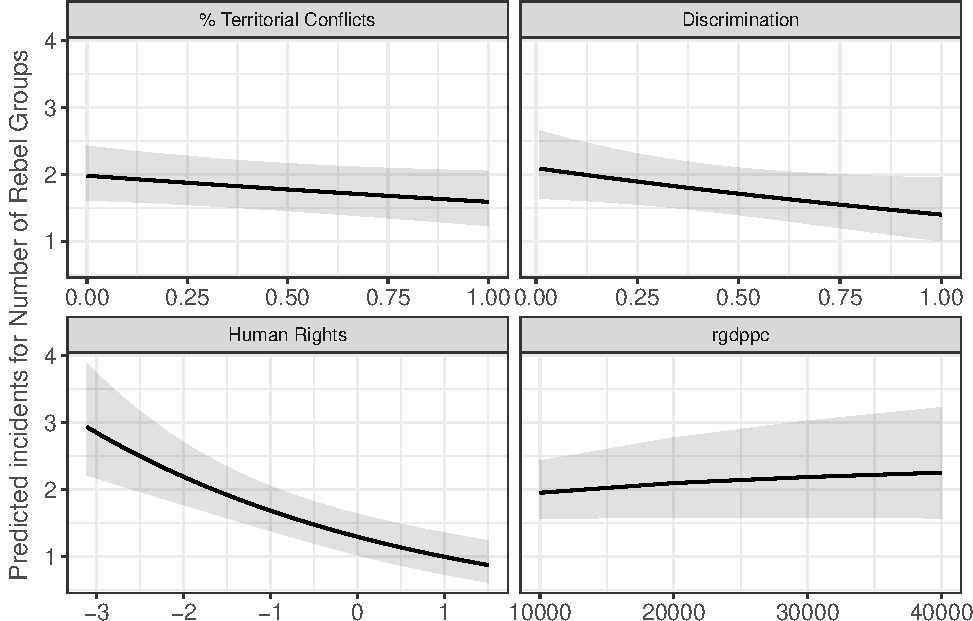
\includegraphics{_main_files/figure-latex/effectplot-1.pdf}
\caption{\label{fig:effectplot}Effect Plots for Model 1}
\end{figure}

\emph{H3}, which predicts an interactive effect between repression and
discrimination, is tested in Models 2 and 4. In Model 2 the interaction
is positive and statistically signficant at the 99.9\% level. The
marginal effects are plotted in Figure 2. The red line shows the
predicted effect of Human Rights at the lowest observed value (i.e.~the
most repressive). At the lowest values of Discrimination (i.e.~a
perfectly indiscriminate political system) and most repressive values of
Human Rights, the expected number of rebel groups is slightly below 2.
As discrimination increases, however, the effect of repression
increases. When 50\% of the population is subject to discrimination, the
expected number of rebel groups is roughly 2.8. When discrimination is
at its highest, with 99\% of the population being free from political
discrimination, the effect of repression is quite strong, with a
prediction of roughly 4.3 rebel groups. At the highest observed levels
of human rights, the expected number of rebel groups is consistently
around 1, and not affected by the level of Discrimination. In short, the
interaction result suggests that we should see the greatest number of
rebel groups when governments use strongly repressive tactics, but
deploy such repression in a highly targeted fashion. When used
indiscriminately, repression has little effect on the number of rebel
groups. In Model 4, the interaction term is just shy of statistical
significance. This suggests that splintering accounts for some of the
interaction effect.

\begin{figure}
\centering
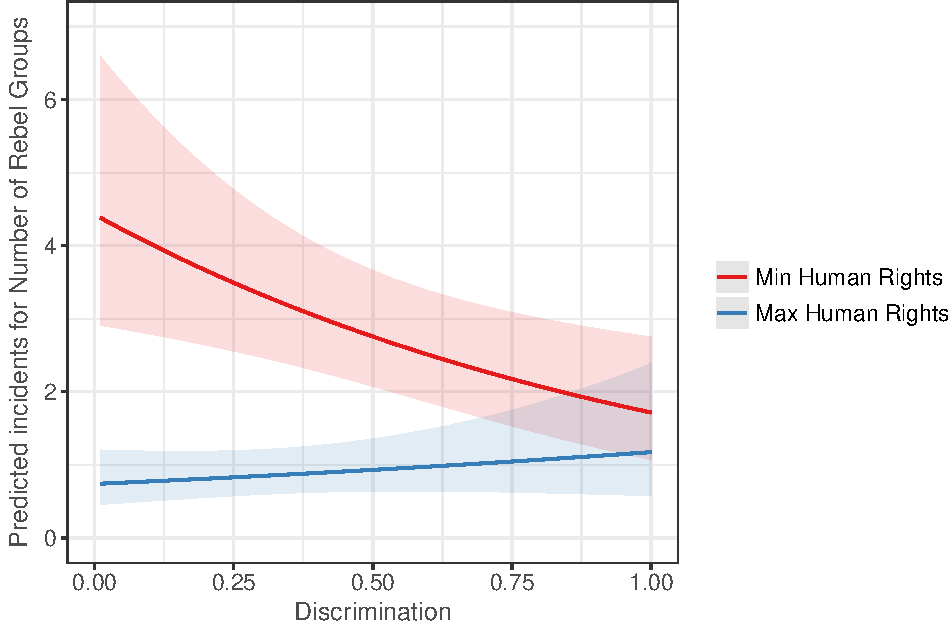
\includegraphics{_main_files/figure-latex/interactionplot-1.pdf}
\caption{\label{fig:interactionplot}Marginal Effects Plots for Repression X
Discrimination Interaction (Model 2)}
\end{figure}

While the results are largely consistent with my hypotheses, this
analysis does have limitations. Perhaps most notably, it does not use a
perfect measure of targeted repression, instead relying on political
discrimination as a proxy. I would argue, however, that this limitations
is more likely to create bias \emph{against} my hypotheses than for
them. There may be people who are not part of an excluded minority
group, but nevertheless are subjected to human rights violations.
Indeed, as factors such as judicial independence and press freedom are
significant components of the Latent Human Rights Scores, such patterns
are likely. In such a case my measure would detect discrimination, but
there would be many individuals behaving as if repression was
indiscriminate. Conversely, some individuals may face limited political
opportunities as a result of discrimination against their ethnic group,
while avoiding threats to their physical integrity. This combination
should produce individuals who are discinclined to cooperate with other
members of society, but are not especially incentivized to resort to
violence due to the absence of physical repression. Nevertheless, more
precise measures should be pursued.

Additionally, this analysis does not facilitate causal claims. It is
possible that government repression strategy is endogenous to the
expectation that multiple rebel groups will emerge, for example. While
lagging the repression and discrimination variables may mitigate this
concern slightly, the addition of an instrumental variable or other
quasi-experimental technique would greatly improve the validity of the
analysis.

\section{Conclusion}\label{conclusion}

I have argued that targeted repression should increase the number of
rebel groups active in a civil war by reducing the relative cost of
participation in rebellion, and by activating ethnic and other
subnational identities that provoke divisions among dissidents. In my
empirical analyses I find support for this theory, as both repression
and discrimination are associated with an increase in the expected
number of rebel groups in a conflict. Furthermore, an interaction effect
shows that repression has the greatest effect on the number of rebel
groups when it is most targeted.

These results suggest that the government plays a surprisingly large
role in shaping rebel movement structure. Existing work on rebel
structure tends to focus on the social context from which rebels emerge
\citep{Staniland2014}, and studies that do consider the role of the
government have often found that repression increases cohesion among
target groups \citep{Simmel1955}, though the effect may be contingent on
internal group dynamics \citep{McLauchlin2012}. Future work should
examine the government's strategic calculus in more detail. My theory
gives little agency to the government, treating as a largely exogenous
source of repression. While it is quite plausible that governments would
prefer to fight a divided opponent rather than a unified one, my theory
and findings suggest that the source of this division is often new
individuals entering the conflict. As this is a seemingly undesirable
outcome, the government's use of targeted repression in conflict
settings is puzzling.

There are also significant opportunities for methodological improvements
to this line of research. First, my empirical analysis does not directly
test my theoretical mechanism - the reorientation of individuals away
from national identities and toward ethnic and other subnational ones.
Survey or experimental research on individuals who have been targeted by
repression would provide a much more direct test of the mechanism.
Additionally, a better measure of targeted repression would improve the
validity of the study. It may be possible to construct such a measure
from geocoded events data. Finally, an instrumental variable or other
causal inference technique would greatly improve the analysis.

A final direction for new research would examine the relationship
between original and joining rebel groups. If my theory is correct,
joining groups should tend to have different ethnic make-ups, and likely
a stronger emphasis on ethnic identity than originating groups. I do not
make any predictions about the relationship between rebel groups when
multiple are present. Surprisingly few works explore conflict between
rebel groups \citep[but see][]{Fjelde2012}, nor do many explore
alliances between rebels \citep[but see][]{Bapat2012}. If the results
presented here are to be believed, such work will be relevant so long as
governments repress.

\chapter{Alliance Formation}\label{alliance-formation-1}

\section{Introduction}\label{introduction-2}

Theories of civil war tend to focus on individual- or group-level
motives \citep[e.g.][]{gurr70, Collier2004} or opportunities
\citep[e.g.][]{fearonlaitin03} for rebellion, while giving little
attention to the organization of dissent into rebel groups and
coalitions. Even those studies which do explicitly consider rebel group
formation tend to focus on group attributes such as discipline
\citep[e.g.][]{Weinstein2007}, and do not consider the possibility that
rebels do not always form a single group. Yet, 44\% of civil conflicts
feature at least two rebel groups challenging the government.\footnote{Source:
  \citet{Pettersson2015a}.} Over the course of the Chadian Civil War,
for instance, 25 distinct rebel groups fought against the government.
Conflicts in Afghanistan in the 1980's, Somalia in the 1990's, and Sudan
in the 2000's have been similarly complex. The ongoing civil war in
Syria is contested by at least two dozen armed groups. Even
ethnically-homogeneous, geographically-concentrated movements with
common goals, such as the Karen secessionist campaign in Myanmar, often
fragment into multiple rebel groups. Furthermore, the number of groups
operating in these conflicts often varies greatly over time. The
existing literature offers many useful insights to the conditions under
which civil war will emerge, but it has few explanations of the
structure of rebel movements.

While little attention has been given to the sources of rebel movement
structure, several studies suggest that such configurations can have
deleterious consequences. Conflicts with multiple rebel groups last
longer than dyadic competitions
\citep{Cunningham2006, Cunningham2009, Akcinaroglu2012a}. Furthermore,
\citet{Cunningham2009} find that the presence of multiple
government-rebel dyads decreases the likelihood of peace agreements and
increases the likelihood of rebel victories, though \citet{Findley2012},
find that fragmented rebel movements are often associated with an
\emph{increased} likelihood of negotiated settlement. Relatedly,
\citet{Atlas1999} and \citet{Zeigler2016} find that episodes of conflict
renewal often occur between formerly allied rebel factions. Finally,
conflicts with multiple dyads feature more fatalities than dyadic
ones.\footnote{Source: my own analysis using data from
  \citet{Sundberg2008a}.} Clearly, conflicts with multiple rebel groups
comprise one of the most severe subsets of civil wars. Thus,
understanding the causes of multi-dyadic conflict is of great normative
and policy importance.

I seek to address this gap by explaining one of the primary determinants
of rebel movement structure --- the formation of alliances between rebel
factions. Which rebel groups are likely to form alliances? With whom are
they likely to ally? While alliances cannot account for all of the
variation in the number of rebel groups in a conflict --- the
fragmentation of existing groups and the entry of previously non-violent
groups to the conflict are also important processes --- alliance ties
tend to predict deeper integration between rebel groups. Many rebel
alliances evolve into umbrella organizations with shared command, and
weak rebel groups are frequently absorbed by alliance partners. Thus,
alliance formation is a crucial determinant of whether conflicts become
less complex over time.

First and foremost, this work advances our understanding of the
complexity of civil conflict in terms of the number and arrangement of
actors. This builds on the growing literature on another facet of
complexity --- the fragmentation of existing groups
\citep[see][]{Cunningham2009, Pearlman2011a, Staniland2014} --- and
presents contrasting evidence to the few existing studies of rebel
alliances \citep{Christia2012, Bapat2012}, which focus on relative
capability as the key driver of coalition building. Furthermore,
examining the relationships between rebel groups sheds new light on
debates about the motives behind rebellion \citep[e.g.][]{Collier2004}.
For instance, if rebellion is fundamentally about ethnic or religious
grievances, we might expect to see the emergence of coalitions with
homogeneous identities. If, by contrast, rebels are motivated by the
desire for profits from natural resources or illicit activities, we
might see groups with access to such revenues seek to limit the number
of combatants with whom they share their spoils, irrespective of common
identity.

I proceed with a review of the literature on relations between rebel
groups. Next, I outline the potential benefits rebels might receive by
forming alliances. Subsequently, I explore the conditions under which
rebels will elect to engage in such cooperation. Finally, I present
results from an inferential network model applied to the Syrian Civil
War.

\section{Relations Among Rebels}\label{relations-among-rebels}

Relations among rebel groups remains one of the most underexplored
aspects of civil war. The vast majority of existing studies focus on
conflict between non-state actors. A few studies have, however, examined
conflict between rebel groups. In the most comprehensive study to date,
\citet{Fjelde2012} suggest that rebels fight each other for control over
resources such drug supplies or valuable terrain. Greater resource
endowments should lead to better postwar bargains with the government in
the long run, and greater ability to sustain a rebellion in the short
run. The authors find that this logic is most likely to prevail in the
presence of natural resources, territories that are not controlled by
the government, militarily weak governments, and significant power
asymmetries among rebels. \citet{Atlas1999} and \citet{Zeigler2016} find
that this dynamic can also arise in the aftermath of conflicts, as the
main fighting in renewed civil wars is often between previously allied
rebel groups.

Another strand of literature examines the emergence of conflict within
previously coherent movements. \citet{Bakke2012a} conceptualize the
fragmentation of rebels movements as varying in terms of the raw number
of organizations, the degree of institutionalization unifying the
organizations, and the distribution of power among them. They expect a
greater general likelihood of infighting in more fragmented movements,
particularly those with large numbers of groups and low degrees of
institutionalization. \citet{Asal2012} find evidence that largely
supports this claim, showing that ethnopolitical movements with
factionalized leadership structures are most likely to experience
splits. Similarly, \citet{Cunningham2012a} find that infighting is most
likely in self-determination movements with large numbers of factions,
and that the emergence of new factions is especially likely to trigger
violence. \citet{Staniland2014} similarly emphasizes pre-existing social
structure, arguing that the probability of an insurgent group
splintering is shaped by the strength of social ties in the organization
from which it emerged. Others see infighting as contingent on the
conflict process. \citet{Christia2012} finds that rebel groups and
coalitions tend to fragment when battlefield losses exacerbate divisions
between faction leaders, while \citet{McLauchlin2012} find that
repression can deepen rifts within movements that are already divided,
but cohesive movements may become further solidified by repression.

There is also a substantial literature on intra-ethnic violence.
\citet{Lilja2011} find that that Tamil rebels used violence against
co-ethnic civilians to control populations and the resources they hold,
and against coethnic armed groups to establish dominance within the
ethnic group. \citet{Staniland2012d} finds that these patterns
intra-ethnic violence tend to be self-reinforcing, as violence within
ethnic insurgencies is the primary cause of the defection of some
subsets of ethnic groups to the opposing side in the conflict.
\citep{Warren2015} seek to explain which ethnic groups are likely to
experience such fragmentation, finding a curvilinear relationship
between the size of an ethnic group and its probably of experiencing
infighting. Small ethnic groups have the ability to police themselves,
limiting violence, and intra-ethnic violence in large groups is likely
to be met with government intervention. Thus, only moderate-sized groups
tend to experience internal violence.

Finally, a few studies consider the formation of alliances among various
types of militant organizations. \citet{Asal2008} and
\citet{Horowitz2013} conduct network analyses of alliance formation
among terrorist groups, arguing that such arrangement are used to
aggregate capabilities and share tactics. \citet{Bapat2012} model the
logic of alliance formation among rebel groups. They assume that
alliances carry two significant costs: the dilution of each constituent
group's agenda, and the risk of having one's private information sold to
the government by an ally. Consistent with this theory, they find
alliances to be most common when an outside state can enforce
agreements, and when all rebel groups involved are strong enough to
avoid the temptation of defecting to the government side
\citet{Christia2012} similarly emphasizes capability, arguing that
neorealist balancing theory from international relations explains
alignments in civil wars. When one coalition - a group of rebels or
government-aligned forces - becomes too powerful, other groups will band
together to prevent their own destruction. But similar
\citet{Bapat2012}, \citet{Christia2012} argues that this mechanism is
constrained by a desire to maximize one's share of the post-war spoils.
Thus, rebels realign frequently, seeking to form minimum winning
coalitions. While shared identity appears on the surface to be an
important determinant of rebel alignments, Christia views these
narratives as post-hoc justifications aimed at legitimizing decisions
that are really driven mostly by power. Some important aspects of
alliance formation are beyond the scope of the existing studies,
however. Namely, while relative power considerations can potentially
account for why rebel groups form alliances, and when they will alter
their ties, it does not explain why groups choose a particular partner
when multiple options are available. Christia suggests that these
decisions are shaped by personal relationships between rebel elites, but
does not give this question extended consideration in her empirical
analysis. \citet{Horowitz2013} find that militants prefer to ally with
powerful groups, but their focus is largely on transnational networks of
terrorists and insurgents, rather than alliance formation within a
particular conflict. I seek to resolve this gap by explaining not only
whether, but also with whom rebel groups will choose to form alliances.

\section{A Theory of Rebel Alliance
Formation}\label{a-theory-of-rebel-alliance-formation}

\subsection{Rebel Factions and Their
Interests}\label{rebel-factions-and-their-interests}

I start from the assumption that governments in civil wars are opposed
by one or more dissident factions. I define a faction as a set of people
with relatively homogeneous beliefs and identities, that is capable of
acting as a group. For example, a communist party might have Leninist
and Maoist factions, and an ethnonationalist movement might have
Christian and Muslim factions. Faction members likely will not share
identical beliefs on every political question, and may not have
identical racial, ethnic, or religious backgrounds. This might be
especially true of factions organized around loyalty to a specific
individual or locale. A faction will, however, tend to be unified on the
most salient political and identity issues of the moment.

In some contexts, the faction may not be an appropriate unit of
analysis. For example, rebel groups often do engage in recruiting new
members on an individual basis, and an individual-level approach would
be appropriate for studying such a phenomenon. For the formation and
restructuring of rebel groups, however, decisions tend to be made by
collectives. \citet{Staniland2014} argues that rebel groups tend to
emerge from existing organizations, rather than spontaneous collections
of individuals. My own data collection shows similar patterns, with 97\%
of rebel groups since 1946 having origins in a pre-existing
organization. When rebel groups fragment, abandonment of the existing
group is often done by entire sub-units. For example
\citet{Staniland2014} finds that fragmentation often takes the form of
local brigades breaking away from a central organization, as was the
case for with al-Qaeda in Iraq, which saw many local Sunni militias
defect and begin cooperating with the US. Similarly,
\citet{Christia2012} sees realignment as being driven by mid-level rebel
commanders, who generally take a cadre of loyal forces with them when
initiating and breaking alliances.

Factions can structured in a variety of arrangements during a conflict.
A faction can resort to violence on an individual basis, resulting in a
rebel group with mostly homogeneous preferences and identities. In other
cases a faction may ally with others to former a larger, but more
heterogeneous rebel group. Finally, factions may remain non-violent,
using peaceful tactics to oppose the government. These arrangement are
dynamic, however. Previously independent factions may form alliances,
previusly aligned factions may choose to break alliances, previously
non-violent factions may choose to enter a conflict, and previously
violent factions may choose to demobilize. I argue that two broad
concerns shape each these decisions.

First, I assume that factions have genuine political interests. This
assumption is not necessarily obvious in light of the long-running
debate as to whether rebellion is motivated by public or private
concerns \citep[see][]{Collier2004}. Indeed, some scholars have gone as
far as to posit that rebellion is little more than glorified criminal
activity aimed at controlling natural resources and illicit trades
\citep{mueller00}, or that individual participation is often motivated
by a desire to settle personal disputes \citep{Kalyvas2006}. I do not
reject the notion that rebels value such things (indeed, see the second
assumption below); I simply contend that greed and grievance are a false
dichotomy. Most rebel groups articulate a political platform of some
variety. This might take the form of a comprehensive ideological program
such as a communist revolution, or a more narrow concern such as land
reform or self-determination for a particular ethnic group. While
earlier work found greater support for the greed hypothesis, suggesting
that such political rhetoric is merely a veneer on more selfish motives,
recent studies using higher-quality data have found that political
grievances, and particularly ethnic discrimination, to be among the
strongest predictors of civil war \citep{Cederman2010}.

Second, however, I expect that factions will seek to maximize their
individual power. Even if rebels are primarily motivated by political
interests, material resources are an important means to achieving such
goals. A faction's influence in any postwar order is likely to be shaped
in large part by its power. If a faction retains enough fighting
capability to re-open violence, other actors interested in peace will
have an interest in accommodating many of their demands. Relatedly, a
faction will have difficulty trusting any concessions it wins from more
powerful actors. Thus, retaining capability at the end of a conflict is
likely to be advantageous with respect to advancing one's political
goals \citep{Nygard2014}. Furthermore, greater power allows a faction
greater autonomy from fellow rebels. Political power is a finite good,
and as a group's capabilities increase, the number of other rebels with
whom they must share it decreases \citep{Christia2012, Bapat2012}.
Finally, even if it is not their primary motive, rebels do use material
resources to incentivize recruitment and retention efforts
\citep{Weinstein2007}, and to enrich top leadership.

\subsection{The Value of Rebel
Alliances}\label{the-value-of-rebel-alliances}

Frequently, rebel factions engage in military collaboration with other
non-state actors. This can range from an agreement not to target each
other, to a divisions of territory, to joint campaigns on the
battlefield, to full mergers. These alliances can be valuable for a
number of reasons. First, alliances aggregate capabilities. This is
perhaps the most common conception of alliances in international
politics \citep[see][]{Bennett1997}, and it has been proposed as a
motive for rebel alliances as well {[}\citet{Bapat2012};
\citet{Horowitz2013}. The logic of capability aggregation differs
somewhat between international and civil conflicts. Whereas
international alliances aggregate capabilities by bringing states into a
conflict in which they might not otherwise participate, rebel groups by
definition are already participating in conflict. Nevertheless, these
alliances can bring great value because rather than simply aggregating,
they can concentrate capabilities in space and time. For example, two
rebel groups might be unable to capture a government-held town on their
own, but in a joint operation would be sufficiently powerful to do so.

Second, alliances can allow for burden-sharing and specialization.
Burden-sharing has been offered as an explanation for international
alliances such as NATO \citep{Sandler1980}, though it may not occur
under all circumstances \citep[see][]{Olson1966}. Alliances can ensure
that a single rebel group is not responsible for defeating the
government, and might serve as a mechanism for reigning in the
temptation to free ride off of another group's efforts. Relatedly,
alliances can facilitate specialization by rebel groups. For instance,
one alliance partner might specialize in holding territory, while
another specializes in launching offensives in new areas. Furthermore,
they can share strategies and technical information. For example, Hamas
is believed to have learned how to use suicide bombings through its
alliance with Hezbollah \citep{Horowitz2013}.

Third, alliances can manage conflict between members and ensure that
their resources are directed toward common enemies. \citet{Weitsman1997}
argues that alliances often serve to tether powerful states to one
another, so as to reduce the probability of conflict between them.
\citet{Gibler1996} finds that alliance treaties are often used to settle
territorial disputes between the signatories. Similar alliances can be
seen in civil wars, for example as a number of Syrian rebel groups
agreed to focus their efforts in different regions of the country. This
allows rebels to avoid conflict with each other. Compliance with such
agreements is incentivized by the fact that reneging on the territorial
arrangement would likely result in the loss of the other benefits of the
alliance, such as capability aggregation.

Fourth, operating as an alliance bloc may be beneficial to the members
groups in bargaining situations. An alliance with a set of coordinated
demands might command greater bargaining leverage than individual
members, who collectively have similar power, but a more disparate set
of demands. Perhaps more crucially, alliances might mitigate credible
commitment problems. Peaceful settlements to conflicts can be derailed
by concerns that the other side will not adhere to the agreement
\citep{fearon95}. In civil wars, this is often borne out by extreme
``spoiler'' factions. A rebel commitment to a peace agreement is more
likely to be viewed as credible if it has formal control over other
factions.

\subsection{The Costs of Alliances}\label{the-costs-of-alliances}

While the benefits are often many, most alliances between rebel groups
are not without cost. The post-war political outcome, whether it comes
in the form of a rebel victory or a compromise with the incumbent
government, is likely to be shaped by all factions within the winning
coalition. Thus, allying with another group holding differing ideologies
and interests will tend to force a rebel faction to compromise on at
least some issues, or to de-emphasize certain priorities. If, as I
assume, rebels are motivated by political goals, the value of an
alliance will decrease as its ideological similarity to its alliance
partners decreases \citep{Bapat2012}. Furthermore, any private benefits
deriving from the conflict outcome (such as seats in a post-war
legistlature) must be divided among the members of the winning alliance
\citep{Christia2012}. These concerns should tend to constrain the value
of alliances in civil war. The existing literature finds that these
concerns limit the size of rebel coalitions \citep{Christia2012}.
Logically, they should also shape the choice of partners with whom
rebels ally.

\subsection{The Choice of Alliance
Partners}\label{the-choice-of-alliance-partners}

I expect that the decision to form an alliance with a particular group
is shaped by two broad considerations. The first is the ideological
similarity of the two groups. The second is the potential gain in
capability. Consistent with the existing literature, I view the current
material capabilities of a potential ally as a crucial factor, with more
powerful groups making more attractive alliance partners. I depart from
the literature \citep[e.g.][]{Christia2012}, however, by also
considering the importance of access to future sources of power.
Specifically, I expect that a group will evaluate a potential alliance
partner not only on its current level of capability, but also on the
extent to which the group is a rival for access to future sources of
power, such as natural resources or civilian populations. In other
words, a rebel group with enough power to normally be an attractive
partner may not be if it's strength is drawn from similar support bases
as one's own group. By contrast, a relatively weak group with a
completely non-overlapping support base might be an attractive ally.

A rebel group's support base is shaped by a mix of external factors such
as the presence of natural resources and foreign sponsors, as well as
its objectives. Some ideological objectives provide rebel groups with
somewhat malleable support bases, such as those that entail the
provision of public, non-rival goods to society. It is comparatively
easy for groups of this sort to minimize the overlap between their
support bases. By contrast, rebels that pursue private, rival goods or
interests specific to certain societal groups are likely to be in
competition with rebels advancing similar objectives. In the remainder
of this section I classify various rebel objectives on this dimension.

Most non-sectarian ideological interests should fall into the category
of public, non-rival goods. If two groups each prefer a similar goal,
such as a redistributive welfare system, a greater role for Islam in
government, or a devolution of power to regional governments, they will
be able to enjoy the benefits of such policies regardless of which group
enacts them. All else equal, goals of this sort should create common
interests among the rebels who share them. Furthermore, policies of this
sort tend not to have pre-defined constituencies. A rebel group based on
ideology could potential convert new members or civilian supporters to
its cause by spreading its beliefs. As ideologies of this sort are
generally not tied to a specific ethnicity, religion, or geographic
area, the pool of potential converts is quite large. Thus, groups
centered around ideologies of this sort should have high potential for
cooperation, as they are relatively unlikely to be rivals for support.
The value of cooperation will be especially high for groups that have
similar non-sectarian ideologies.

\emph{H1: Rebel groups with similar non-sectarian ideologies should be
more likely to form alliances than other rebel dyads}

While groups with similar non-sectarian interests should tend not to
come into competition until late in conflicts, for groups representing
identity-based interests, the effect is contingent on the size of the
group and malleability of group boundaries. The reason for this lies in
the fact that many rebel groups rely on civilian populations for
material support \citep{Weinstein2007}, and the types of goals a group
pursues is an important determinant of the malleability of civilian
support coalitions. A group with broad-based policy goals might be able
to persuade or coerce almost any group of citizens to support it. Thus,
until a very large portion of the civilian population has been captured,
groups sharing these types of goals will not be in competition over
support as they can simply carve out different coalitions. Similar
dynamics should occur among groups pursuing the interests of large or
social groups, such as the majority ethnic or religious group. For
example two Syrian rebel groups seeking to replace the Alawite-dominated
Assad regime with one that embraces Sunni doctrine should find that
civilian support is not particularly scarce given that Syria is
majority-Sunni. Similarly, groups advocating the interests of social
groups with fluid boundaries should tend to have opportunities to
capture new civilian support rather than competing with similar groups
over existing support. For instance, for a group advocating a
Salafi-Jihadi ideology, any Sunni Muslim might serve as a potential
convert.

Rebels representing minority social groups, however, should tend to come
into conflict more quickly. Groups of this sort must draw their support
from a social base that is both smaller and more likely to be tapped out
than the bases of more broadly defined groups, and that is more rigidly
bounded. A rebel group aimed at advancing the interests of a particular
ethnic or religious group is unlikely to attract support from non-group
members. Even if it was able to do so, this might its standing with
co-ethnics/co-religionists, as rival groups could claim that it is
watering down its agenda. In other words, socially-defined rebel groups
seeking to expand the pool of potential support might be vulnerable to
outbidding appeals. In short, I expect that groups with the agenda of
advancing the interests of majority ethnic or religious groups will be
likely to cooperate with groups holding similar interests. Groups
representing social minorities, however, should be unlikely to
cooperate.\footnote{In the present analysis, however, the Kurds are the
  only group to whom this logic is likely to apply, and thus I do not
  test this hypothesis as it would essentially be a dummy variable for
  the one Kurdish-Kurdish dyad.}

\emph{H2: Rebel groups representing the same majority ethnic or
religious groups will be more likely to form alliances than other dyads}

Groups seeking to control the same territory should face a similar
problem of rival consumption. Because secessionist claims tend to have
well-defined geographic and/or ethnic boundaries, rebel groups
representing such claims are likely to be in competition over a fixed
pool of support. Thus, I expect that groups making similar territorial
claims will be unlikely to cooperate.

\emph{H3: Rebel groups with overlapping territorial claims will be less
likely to form alliances than other dyads}

\section{Conclusion}\label{conclusion-1}

I have argued that contrary to some theoretical treatments, rebel groups
do care about political aims. This fact should lead alliance ties to be
most common among groups sharing similar goals. Indeed, I find that in
the Syrian Civil War, shared political goals are the single most
important determinant of alliance partners. I do not find support for
the notion that more powerful groups should be more likely to form
alliances. While I do not find evidence of religious homophily, that may
be an artifact of the limited diversity of Syrian rebels. Finally, I
find a null relationship between shared territorial ambitions and
alliances, where I expected a negative relationship.

The finding on the importance of political goals contrasts with multiple
existing theories of rebellion. The importance of political goals
contrasts with the greed model of civil war, which views rebellion as
being primarily aimed at procuring private material benefits for
members. It also calls into question purely power-based accounts
\citep{Christia2012}, which expect rebels to be concerned with little
else but winning. In addition, these results can help us to predict the
dynamics of civil conflicts. If we observe a conflict with many rebel
factions, but these groups share similar goals, we might expect the
movement to aggregate over time. If these groups have disparate
interests, however, there is a strong possibility that the conflict will
remain highly fragmented. Given the severity associated with more
complex conflicts, the ability to make predictions of this sort is
highly valuable.

Further research in this area is needed. My hypothesized effects may
simply be conditional on factors that I have yet to account for. For
example, access to material support from an outside actor should reduce
competition over civilian support bases or territory. In addition, this
work should be replicated in other cases. As one of the most complex
civil wars on record, it is possible that the dynamics in Syria do not
apply in other conflicts. Finally, future work should move beyond
explaining the formation of networks and explore the effects of network
structure on rebel behavior. For instance, are more densely networked
rebel coalitions more resilient to anti-insurgent campaigns? Do certain
tactics diffuse across rebel networks?

\chapter*{References}\label{references}
\addcontentsline{toc}{chapter}{References}

\indent

\setlength{\parindent}{-0.2in} \setlength{\leftskip}{0.2in}
\setlength{\parskip}{8pt}

\singlespacing

\bibliography{/Users/david/Dropbox/library.bib}


\end{document}
